\documentclass{article}
\usepackage[utf8]{inputenc}
\usepackage[a4paper, total={7in, 8in}]{geometry}
\usepackage{fancyhdr}
\usepackage{pdfpages}
\usepackage{lastpage}
 
 


\pagestyle{fancy}
\fancyhf{}
\fancyhead[L]{Grid-World project report}
\rfoot{Page \thepage \hspace{1pt} of \pageref{LastPage}}

\title{\textbf{Project GridWorld\\Final Report}}
\author{Stavros Orfanoudakis 2015030030 \\ Andreas Kallinteris 	2017030066}
\date{\today}

\usepackage{natbib}
\usepackage{graphicx}

\begin{document}

\maketitle

\section{Introduction}
In the following project we are going to study some search algorithms in a 2-D grid-world like space. Specifically, our agent has to reach it's destination considering two kind of walkable tiles (grass and land) and one unwalkable obstacle tile (wall). To do that we had to implement BFS, DFS , A* and LRTA* algorithms in order to test which one behaves better.

\section{Implementation}
In this section we are going to explain the implementation of each separate algorithm.

\subsection{DFS}
    DFS algorithm has been implemented as a stack , which means that our agent picks one non-discovered neighbouring node and expand ,while at the same time it puts the rest neighbouring nodes within the stack.This is repeated until the agent reach the destination. In particular, when expanding nodes, we have to make sure that the nodes ,at first are within the borders of the grid and secondly that the node is not a wall.
\subsection{BFS}
    BFS algorithm adds all it's neighbouring non-discovered nodes into a queue and always expands the first in priority node .BFS keeps expanding considering the previous constraints, until it reaches the final destination.
\subsection{A*}
    A* search algorithm has been implemented as following. At first we initialize an $nxn$ "discovered" table so we can store the cost estimation of each node .Later the agent puts every neighbouring node ,that is not discovered yet or has a cost estimate lower than the previous one, in a buffer where each node has index and weight.After that, it checks every node in the buffer and returns the one with the lowest weight so the agent can move there. These actions are going to be repeated until the agent reaches the destination. When the agent reaches the destination the "discovered" table would be filled with useful values that are going to provide us (through backtracking) the optimal path. \\
    Also it is worth mentioning ,how the cost of every node is estimated. Each weight comes from this function $f(n) = g(n) + h(n)$ where $g(n)$ is the cost from the start to the n node and $h(n)$ is the heuristic function which estimates the distance to the destination. Regarding the heuristic function ,we tested a variety of functions and we ended up at the point where we found that the Manhattan distance is better most of the times, like bibliography suggested .
\subsection{LRTA*}
    Learning real time A* is a local search algorithm. This algorithm is special ,because the weight of the node is determined after the agent walk there himself. This makes the problem a bit harder to solve. In our implementation we used the following LRTA* code.


\begin{figure}[h!]
\centering
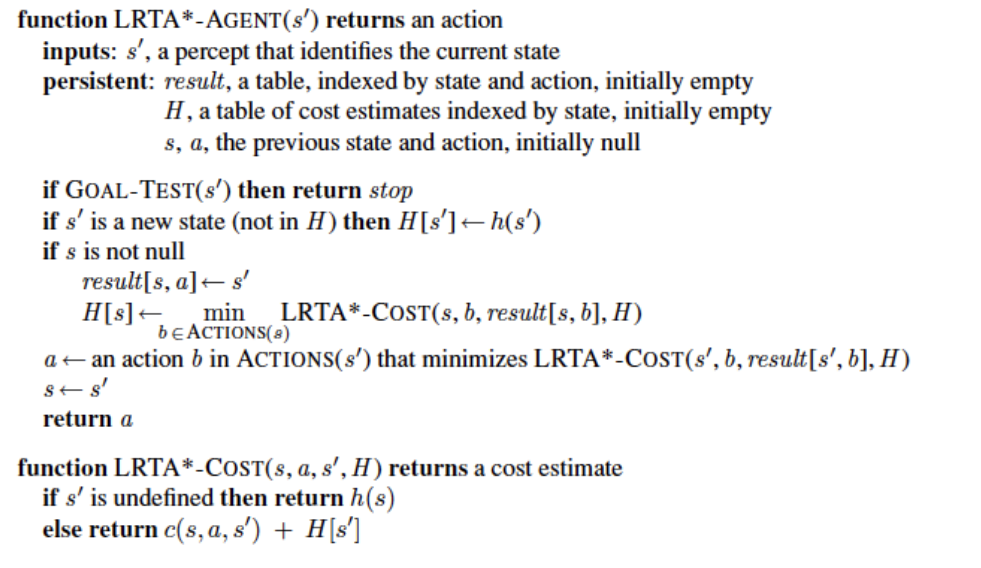
\includegraphics[scale=0.5]{lrta.png}
\end{figure}
    It is worth saying ,that when there are two or more actions that minimize the LRTA* cost, we choosed the node which where closer to the destination using the same heuristic function as A* ( Manhattan distance).
    
    
\section{Evaluation - Results}
    In the following section we are going to present the results , after running each algorithm in 5 given worlds with grass cost 2 and 5.
\subsection{BFS}   
Below we can see the \textbf{path steps} it took BFS algorithm to reach destination.
\begin{table}[!htb]
\centering
\begin{tabular}{|c|c|c|c|c|c|}
\hline
\textit{\textbf{BFS}} & \textbf{easy} & \textbf{default} & \textbf{hard\_a} & \textbf{hard\_b} & \textbf{hard\_c} \\ \hline
\textbf{grass\_cost : 2, 5} & 55 & 36 & 87 & 86 & 123 \\ \hline
\end{tabular}
\end{table}

\subsection{DFS}
Below we can see the \textbf{path steps} it took DFS algorithm to reach destination.

\begin{table}[!htb]
\centering
\begin{tabular}{|c|c|c|c|c|c|}
\hline
\textbf{DFS}              & \textbf{easy} & \textbf{default} & \textbf{hard\_a} & \textbf{hard\_b} & \textbf{hard\_c} \\ \hline
\textbf{grass\_cost : 2, 5} & 48            & 71               & 118              & 112              & 198              \\ \hline
\end{tabular}
\end{table}
\subsection{A*}
Below we can see the cost of the optimal path and the number of steps it requires, using A*.
\begin{table}[!htb]
\centering
\begin{tabular}{|c|c|c|c|c|c|}
\hline
\textit{\textbf{A*}} & \textbf{easy} & \textbf{default} & \textbf{hard\_a} & \textbf{hard\_b} & \textbf{hard\_c} \\ \hline
\textbf{grass\_cost :2} & 11 (11 steps) & 15 (8 steps) & 20 (17 steps) & 19 (16 steps) & 24 (20 steps) \\ \hline
\multicolumn{1}{|l|}{\textbf{grass\_cost : 5}} & \multicolumn{1}{l|}{11 (11 steps)} & \multicolumn{1}{l|}{24(20 steps)} & \multicolumn{1}{l|}{23 (23 steps)} & \multicolumn{1}{l|}{28 (16 steps)} & \multicolumn{1}{l|}{32 (28 steps)} \\ \hline
\end{tabular}
\end{table}

\subsection{LRTA*}
Below we can see the cost of the path and the number of steps it requires, using LRTA*.

\begin{table}[!htb]
\centering
\begin{tabular}{|c|c|c|c|c|c|}
\hline
\textit{\textbf{LRTA*}} & \textbf{easy} & \textbf{default} & \textbf{hard\_a} & \textbf{hard\_b} & \textbf{hard\_c} \\ \hline
\textbf{grass\_cost :2} & 14 (11 steps) & 15 (8 steps) & 36 (29 steps) & 21 (16 steps) & 48 (42 steps) \\ \hline
\end{tabular}
\end{table}

\subsection{Results}
We can see that DFS and BFS algorithms are the worst considering the path cost , but this is natural ,because these algorithms doesn't consider the weight of the nodes they process. On the other hand A* is optimal and we can prove that through the previous tests. That means that there is no better path than the one discovered by A* agent.
We can also observe ,that the learning real time algorithm doesn't find the overall optimal path like A* , but it can find a very close to optimal path depending on the complexity and the size of the world it searches.
\section*{Code notes}
Our code is implemented in C++ . We use the implemented worlds text files so we can load the worlds to this project. Also ,we used make-file to execute the project through terminal (command \$make cr when in the project folder).Boost C++ library is required for our BFS to run (we use an implemented cyclic buffer to save time).
\end{document}
